\chapter{Généralités}
\label{chap:generalites}

Dans ce premier chapitre, nous donnons la formulation des équations de Maxwell.
Ces équations régissent
la propagation des ondes électromagnétiques et nous permettront
de la modéliser par la simulation numérique.

Nous écrivons ensuite ces équations sous la forme d’un
système hyperbolique symétrique linéaire du premier ordre, aussi appelé système de Friedrichs,
pour lesquels de nombreuses propriétés sont connues.
Nous examinons
ensuite les possibles discontinuités des solutions de ce système
et donnons les condition d'existence et d'unicité d'une
telle solution.

Enfin, nous introduisons la formulation Galerkin Discontinue (GD)
du système hyperbolique ainsi obtenu, en passant par la formulation faible
du problème d'évolution étudié. 
Nous listons alors quelques flux numériques permettant
d'améliorer la stabilité du schéma
et terminons par donner la formulation semi-discrète du problème.
\\


\section{Équations de Maxwell}
\label{sect:equations_de_maxwell}

Les équations de Maxwell décrivent la propagation des champs électromagnétiques
dans un milieu quelconque. À la fin du $\textrm{XIX}^\textrm{ème}$ siècle, le physicien James Clerk Maxwell
s’est basé sur les travaux existants concernant l’électricité et le magnétisme afin
de les unifier en un système de huit équations. Plus tard, Olivier Heaviside les
reformula sous forme de quatre équations aux dérivées partielles
que nous présentons ci-après.
\\

Nous notons $\x = \xDef$ un point de l’espace
$\Esp$ et $\Ptl{i}$ la dérivée partielle suivant $\x_i$. 
De plus, nous notons $\nabla = \nablaDef$
l’opérateur gradient. Les opérateurs rotationnel et divergence
sont respectivement notés $\Rot$ et $\Div$, où $\times$ représente
le produit vectoriel et $\cdot$ le produit scalaire usuel.
La dérivée partielle en temps est notée $\Ptl{t}$.

%  BW: pour parler de dtE, il faut que E dépende du temps et donc que E soit défini de R4 dans R3. Idem pour H
%  PH: écrire que E(x,t) est dans R3, c'est plus simple
%  BW: ok
Soient $\E(\x,t) \in \Esp$ le champ électrique,
$\H(\x,t) \in \Esp$ le champ magnétique,
$\J(\x,t) \in \Esp$ le courant électrique et
$\Dens(\x,t) \in \EnsR$ la densité de charge électrique.
Soient $\EPrm$, $\HPrm$, $\ECnd$ et $\HCnd$ les
paramètres constitutifs des matériaux, représentant respectivement
la permittivité, la perméabilité et les conductivités électrique et magnétique
du milieu. Dans le cas des matériaux linéaires, homogènes, isotropes, et avec réponse
instantanée aux changements du champ électrique, ces paramètres sont des constantes
propres au matériau.

Avec ces notations et en tenant compte des équations constitutives des milieux
linéaires, les équations de Maxwell s’écrivent :
\begin{subequations}
	% D = esilon * E
	% B = mu * H
	\begin{align}
		\Ptl{t} \EPrm \E + \ECnd \E - \Rot \H &= - \J
		\label{eq:maxwell_ampere} ,
		\\
		\Ptl{t} \HPrm \H + \HCnd \H + \Rot \E &= 0
		\label{eq:maxwell_faraday} ,
		\\
		\Div \EPrm \E &= \Dens
		\label{eq:maxwell_gauss} ,
		\\
		\Div \HPrm \H &= 0
		\label{eq:maxwell_thomson} ,
		\\
		\Ptl{t} \Dens + \Div (\J + \ECnd \E) &= 0
		\label{eq:conservation_charge} .
	\end{align}
	\label{eq:maxwell}
\end{subequations}

L’équation \eqref{eq:maxwell_ampere} est appelée équations de Maxwell-Ampère.
Cette équation énonce qu'une variation du champ électrique ou la présence d'un
courant électrique génèrent un champ magnétique. L'équation \eqref{eq:maxwell_faraday}
est appelée équations de Maxwell-Faraday. Cette seconde équation indique que la
variation d'un champ magnétique génère un champ électrique.

À ces deux équations
s’ajoutent des conditions sur les divergences des champs électromagnétiques exprimées
par les équations de Maxwell-Gauss \eqref{eq:maxwell_gauss} et Maxwell-Thomson
\eqref{eq:maxwell_thomson}. Ces équations précisent que le flux électrique sortant
d'un volume est lié à la charge électrique contenue dans ce volume et que le flux
magnétique à travers une surface fermée est nul.

Enfin, la dernière équation \eqref{eq:conservation_charge} donne la propriété de
conservation de la charge électrique.
\\

\begin{proposition} \label{prop:divergence}
	\begin{sloppypar}
	Si les équations de Maxwell-Gauss \eqref{eq:maxwell_gauss} et Maxwell-Thomson
	\eqref{eq:maxwell_thomson} sont vérifiées à l'instant initial pour une solution des
	équations de Maxwell, alors elles sont vérifiées à chaque instant.
	\end{sloppypar}
\end{proposition}

\begin{proof}
	\begin{sloppypar}
	En appliquant l'opérateur divergence aux équations de Maxwell-Ampère
	\eqref{eq:maxwell_ampere} et Maxwell-Faraday \eqref{eq:maxwell_faraday},
	par le fait que la divergence d'un rotationnel est nulle, nous obtenons :
	\end{sloppypar}
	\begin{subequations}
		\begin{align}
			\Ptl{t} \Div \EPrm \E &= - \Div (\J + \ECnd \E)
			\label{eq:maxwell_ampere_div} ,
			\\
			\Ptl{t} \Div \HPrm \H &= - \Div \HCnd \H
			\label{eq:maxwell_faraday_div} .
		\end{align}
	\end{subequations}
	Nous utilisons ensuite l'équation de conservation de la charge
	\eqref{eq:conservation_charge} sur la première 	équation ainsi obtenue
	\eqref{eq:maxwell_ampere_div} et l'équation de Maxwell-Thomson \eqref{eq:maxwell_thomson}
	sur la seconde équation \eqref{eq:maxwell_faraday_div} :
	\begin{subequations}
		\begin{align}
			\Ptl{t} \Div \EPrm \E &= \Ptl{t} \Dens ,
			\\
			\Ptl{t} \Div \HPrm \H &= 0 .
		\end{align}
	\end{subequations}
	Enfin, en appliquant les conditions initiales données par les équations de
	Maxwell-Gauss \eqref{eq:maxwell_gauss} et Maxwell-Thomson \eqref{eq:maxwell_thomson} :
	\begin{subequations}
		\begin{align}
			\Div \EPrm \E (\x,0) &= \Dens (\x,0) ,
			\\
			\Div \HPrm \H (\x,0) &= 0 ,
		\end{align}
	\end{subequations}
	nous obtenons le résultat souhaité.
\end{proof}


%  PH: mal dit: elles sont quand même importantes !!!
%Nous pouvons donc ignorer
%les équations de Maxwell-Gauss et Maxwell-Thomson dans la suite.
%  BW: reformulé
Nous pouvons donc nous contenter de ne considérer que les équations de
Maxwell-Ampère et Maxwell-Faraday dans la suite, en gardant à l'esprit que
les équations de Maxwell-Gauss et Maxwell-Thomson doivent être vérifiées
à l'instant initial du problème considéré.
\\


\section{Système de Friedrichs}
\label{sect:systeme_de_friedrichs}

Nous venons de justifier le fait que, en principe, il suffit de résoudre
les équations de Maxwell-Ampère \eqref{eq:maxwell_ampere} et Maxwell-Faraday
\eqref{eq:maxwell_faraday}.
Dans la suite, nous appellerons le système constitué de ces deux équations
« les équations de Maxwell ». Nous pouvons écrire ces équations sous la forme
plus générique d'un système dit de Friedrichs \cite{friedrichs_definition, friedrichs_courant, friedrichs_ern} afin de bénéficier
des propriétés connues sur ces derniers.
\\

\subsection{Définitions}
\label{ssect:systeme_de_friedrichs_definitions}

%  PH: mettre une définition: un système est de friedrichs si les matrices sont symétriques
%  BW: reformulation de la définition
\begin{definition} \label{def:friedrichs}
	Soit $\W(\x,t)$ un vecteur
	de $\NC$ fonctions solution du système d'équations aux dérivées
	partielles suivant :
	\begin{align}
		\Ptl{t} \At \W + \ACnd \W + \sum_{i=1}^3 \Aidi \W = \Src
		\label{eq:friedrichs}
	\end{align}
	avec $\At$, $\ACnd$ et $(\Ai)_{i \in \Range{1}{3}}$ des matrices carrées
	réelles de taille $\NC$ et $\Src$ un vecteur de $\NC$ fonctions sources.
	Ce système est dit \textbf{de Friedrichs} si pour toute direction
	$\n = \nDef$ de $\Esp$ la matrice $\A = \sum_{i=1}^3 \Aini$ est symétrique
	et si la matrice $\At$ est symétrique et définie positive.
\end{definition}

\begin{notation}
	Dans la suite nous utiliserons la convention de sommation des indices répétés,
	\textit{i.e.} $\sum_{i=1}^3 \Aidi = \Aidi$.
\end{notation}

Dans le cas des équations de Maxwell, le vecteur
$\W = \Trp{(\Trp{\E},\Trp{\H})}$
est le vecteur des champs électromagnétiques avec $\NC = 6$.
Les matrices $\At$, $\ACnd$ et
$(\Ai)_{i \in \Range{1}{3}}$ et le vecteur $\Src$ se déduisent des
équations de Maxwell et valent :

\begin{subequations}
	\begin{align}
		\At =
		\begin{pmatrix}
			\EPrm & 0 & 0 & 0 & 0 & 0 \\
			0 & \EPrm & 0 & 0 & 0 & 0 \\
			0 & 0 & \EPrm & 0 & 0 & 0 \\
			0 & 0 & 0 & \HPrm & 0 & 0 \\
			0 & 0 & 0 & 0 & \HPrm & 0 \\
			0 & 0 & 0 & 0 & 0 & \HPrm
		\end{pmatrix}
		\label{eq:matrice_at} ,
	\end{align}
	\begin{align}
		\ACnd =
		\begin{pmatrix}
			\ECnd & 0 & 0 & 0 & 0 & 0 \\
			0 & \ECnd & 0 & 0 & 0 & 0 \\
			0 & 0 & \ECnd & 0 & 0 & 0 \\
			0 & 0 & 0 & \HCnd & 0 & 0 \\
			0 & 0 & 0 & 0 & \HCnd & 0 \\
			0 & 0 & 0 & 0 & 0 & \HCnd
		\end{pmatrix}
		\label{eq:matrice_sigma} ,
	\end{align}
	\begin{align}
		\Ac{1} =
		\begin{pmatrix}
			0 & 0 & 0 & 0 & 0 & 0 \\
			0 & 0 & 0 & 0 & 0 & 1 \\
			0 & 0 & 0 & 0 & -1 & 0 \\
			0 & 0 & 0 & 0 & 0 & 0 \\
			0 & 0 & -1 & 0 & 0 & 0 \\
			0 & 1 & 0 & 0 & 0 & 0
		\end{pmatrix}
		\label{eq:matrice_a1} ,
	\end{align}
	\begin{align}
		\Ac{2} =
		\begin{pmatrix}
			0 & 0 & 0 & 0 & 0 & -1 \\
			0 & 0 & 0 & 0 & 0 & 0 \\
			0 & 0 & 0 & 1 & 0 & 0 \\
			0 & 0 & 1 & 0 & 0 & 0 \\
			0 & 0 & 0 & 0 & 0 & 0 \\
			-1 & 0 & 0 & 0 & 0 & 0
		\end{pmatrix}
		\label{eq:matrice_a2} ,
	\end{align}
	\begin{align}
		\Ac{3} =
		\begin{pmatrix}
			0 & 0 & 0 & 0 & 1 & 0 \\
			0 & 0 & 0 & -1 & 0 & 0 \\
			0 & 0 & 0 & 0 & 0 & 0 \\
			0 & -1 & 0 & 0 & 0 & 0 \\
			1 & 0 & 0 & 0 & 0 & 0 \\
			0 & 0 & 0 & 0 & 0 & 0
		\end{pmatrix}
		\label{eq:matrice_a3} ,
	\end{align}
	\begin{align}
		\Src = \Trp{\left(-\Trp{\J},\Trp{0_{\Esp}}\right)}
		\label{eq:source} .
	\end{align}
\end{subequations}
Nous constatons que la matrice $\At$ est symétrique définie positive et que les matrices
$\Ai$ sont symétriques. Nous sommes donc bien en présence d'un système de Friedrichs.

La matrice $\Aini$ de la définition \ref{def:friedrichs} est donnée par :
\begin{align}
	\Aini = 
	\begin{pmatrix}
		0 & -\n \times \\
		\n \times & 0
	\end{pmatrix} ,
	\; \mathrm{avec} \;
	\n \times =
	\begin{pmatrix}
		0 & -\nC{3} & \nC{2} \\
		\nC{3} & 0 & -\nC{1} \\
		-\nC{2} & \nC{1} & 0
	\end{pmatrix} .
\end{align}
Les valeurs propres de cette matrice sont $\Norm{\n}^2$, $0$ et
$-\Norm{\n}^2$, chacune de multiplicité $2$.
\\

%  PH: autre définition: système hyperbolique
%  BW:
Nous pouvons aussi énoncer la définition plus générale d'un système hyperbolique
dans $\Esp$ :
%  PH: matrice en gras composante pas en gras
%  BW: ok
\begin{definition}
	Soit $\U(\x,t) =
	\Vect{u_1}{\dots}{u_\NC}$ un vecteur
	de $\NC$ fonctions solution du système d'équations aux dérivées
	partielles suivant :
	\begin{align}
		\Ptl{t} \U + \Ptl{i} f^i(\U) = 0
		\label{eq:systeme_hyperbolique}
	\end{align}
	avec $f^i \in \mathcal{C}^1(\EnsR^\NC,\EnsR^\NC)$ des fonctions
	continuement dérivables non nécessairement linéaires. Soit aussi les matrices
	$\Ai = (\Ptl{u_k} f^i_j)_{j,k \in \Range{1}{\NC}}$.
	Ce système est dit \textbf{hyperbolique} si pour toute direction
	$\n$ de $\Esp$ la matrice $\A = \Aini$ est diagonalisable dans $\EnsR$.
\end{definition}


%  PH: proposition: un système de fridedrichs est hyperbolique
%  BW:
\begin{proposition}
	Un système de Friedrichs est hyperbolique.
\end{proposition}

%  PH: formaliser ainsi la suite :
%  BW: vu
\begin{proof}
	Un système de Friedrichs est hyperbolique si pour toute direction $\n$ de $\Esp$
la matrice $\Inv{\At}\Aini$ est diagonalisable dans $\EnsR$.
Or, la matrice $\At$ est diagonale définie positive et la matrice $\Aini$ est
symétrique et donc diagonalisable dans $\EnsR$.
Il est donc aisé de démontrer que le produit
$\Inv{\At}\Aini$ est diagonalisable et à valeurs propres réelles.
Le système étudié est donc un système hyperbolique.
\end{proof}


\subsection{Condition de saut}
\label{ssect:systeme_de_friedrichs_saut}


%  PH: réserver omega aux ouverts en espace. utiliser Q par exemple pour les ouverts espace temps
%  BW: ok pour Q
Nous allons maintenant examiner les possibles discontinuités apparaissant
dans les solutions du système hyperbolique \eqref{eq:friedrichs}. Les discontinuités
apparaissant dans une solution d’un tel système vérifient les conditions
de saut de Rankine-Hugoniot \cite{sauts}.
Appliquons ces conditions aux équations de Maxwell.



\subsubsection{Relation de Rankine-Hugoniot}
\label{sssect:rankine-hugoniot}

Soit $\PbEsp$ un ouvert de $\Esp$ et $\Tmax$ un réel positif.
Considérons une surface spatio-temporelle régulière
$\PbSrfTps \subset \PbEspTps = \PbEsp \times \PbTps$
orientée par une normale notée
$\tilde{\n} = \Trp{(\Trp{\n},\nC{t})}$ (figure \ref{img:discontinuite}).
Le vecteur unitaire $\n \in \Esp$ est la partie spatiale de la normale et
$\nC{t} \in \EnsR$ est la partie temporelle de la normale.

Cette surface $\PbSrfTps$ sépare $\PbEsp$ en deux ouverts $\PbEsp_\L$ et
$\PbEsp_\R$. Nous supposons que $\n$ est orienté de $\PbEsp_\L$ vers
$\PbEsp_\R$. Notons $\W_\L$, respectivement $\W_\R$, la
restriction des champs électromagnétiques $\W$ à $\PbEsp_\L$, respectivement
$\PbEsp_\R$. $\W_\L$ et $\W_\R$ sont solutions $\mathcal{C}^1$ des
équations de Maxwell et $\W$ vérifie la condition de Rankine-Hugoniot sur la
discontinuité $\PbSrfTps$.

Dans la suite de cette section, l'indice $\L$,
respectivement $\R$, apposé à une notation existante fait référence au côté
$\PbEsp_\L$, respectivement $\PbEsp_\R$, de la discontinuité.

%  PH: mettre un dessin, citer le bouquin de schwartz méthodes math. pour la physique
%  BW: le livre est cité dans le paragraphe précédent = \cite{sauts}

\begin{figure}[h]
	\begin{center}
		\caption{
			\label{img:discontinuite}
			Schéma représentant une discontinuité spatio-temporelle %fixe
			$\PbSrfTps$ dans $\PbEspTps = \PbEsp \times \PbTps$.
		}
		
		\begin{tikzpicture}[scale=1]
			% Axe omega
			\draw[-] (0,0)
				-- node[midway, above] {$\PbEsp_\R$} (3,0)
				-- node[midway, above] {$\PbEsp_\L$}
				(8,0) node[right]{$\PbEsp$};
			
			% Axe t
			\draw[arrows={-latex}] (0,-0.1) -- (0,6) node[above left]{$t$};
			\draw[-] (-0.1,0) node[left]{$0$} -- (0.1,0);
			\draw[-] (-0.1,5.5) node[left]{$\Tmax$} -- (0.1,5.5);
			
			% Normale (coeff th: -0.454545 pr: -0.5)
			\draw[arrows={-latex},red,very thick] (4.5,3.3)
				-- node[red, midway, above right] {$\tilde{\n}$} (2.5,4.3);
			\draw[arrows={-latex},dashed] (4.5,3.3)
				-- node[midway, below] {$\n$} (2.5,3.3);
			\draw[arrows={-latex},dashed] (2.5,3.3)
				-- node[midway, left] {$\nC{t}$} (2.5,4.3);
			
			\draw[dotted] (2.5,0) -- (2.5,3.3);
			\draw[dotted] (4.5,0) -- (4.5,3.3);
			\draw[dotted] (0,3.3) -- (2.5,3.3);
			\draw[dotted] (0,4.3) -- (2.5,4.3);
			
			% angle droit
			\draw[-,red,very thin] (4.3,3.4) -- (4.4,3.62);
			\draw[-,red,very thin] (4.4,3.62) -- (4.6,3.5);
			
			% Discontinuité (coeff 2.2)
			\draw[-,blue] (3,0) -- (5.5,5.5) node[above,blue]{$\PbSrfTps$};
		\end{tikzpicture}
	\end{center}
\end{figure}


%  PH: c'est une définition. ce serait une proposition si tu disais : solution au sens des distributions implique rankine-hugoniot
%  BW: ok pour une définition, n'est-ce pas bizarre un "ssi" dans un définition ?
\begin{definition}
	Soit $\Trp{(\Trp{\n},\nC{t})}$, avec $\n$
	un vecteur unitaire, la normale
	au support d'une discontinuité de la solution du système
	hyperbolique \eqref{eq:friedrichs}.
	La relation de Rankine-Hugoniot satisfaite sur cette discontinuité
	est donnée par l'équation :
	\begin{align}
	\nC{t} \left( (\At)_\L \W_\L - (\At)_\R \W_\R \right) =
	\left( (\Aini)_\L \W_\L - (\Aini)_\R \W_\R \right) ,
	\end{align}
	avec $\nC{t}$ la vitesse de propagation de la discontinuité.
\end{definition}

En appliquant cette relation aux équations de Maxwell, nous déduisons la
propriété suivante :
\begin{proposition}
	De part et d’autre de la discontinuité, les champs vérifient :
	\begin{subequations}
		\begin{align}
		\nC{t} (\EPrm_\L \E_\L - \EPrm_\R \E_\R) &= - \n \times (\H_\L - \H_\R) ,
		\\
		\nC{t} (\HPrm_\L \H_\L - \HPrm_\R \H_\R) &= \n \times (\E_\L - \E_\R) .
		\end{align}
	\end{subequations}
\end{proposition}


\subsubsection{Interprétation}
\label{sssect:rankine-hugoniot_interpretation}

En milieu homogène ($\EPrm_\L = \EPrm_\R = \EPrm$
et $\HPrm_\L = \HPrm_\R = \HPrm$), les équations précédentes
peuvent être écrites sous la forme matricielle :
\begin{align}
	\nC{t}
	\begin{pmatrix}
		\E_\L - \E_\R \\
		\H_\L - \H_\R
	\end{pmatrix} =
	\begin{pmatrix}
		0 & - \frac{1}{\EPrm} \n \times \\
		\frac{1}{\HPrm} \n \times & 0
	\end{pmatrix}
	\begin{pmatrix}
		\E_\L - \E_\R \\
		\H_\L - \H_\R
	\end{pmatrix} .
\end{align}
Le vecteur $\Trp{(\Trp{(\E_\L - \E_\R)}, \Trp{(\H_\L - \H_\R)})}$
est donc vecteur propre associé à la valeur propre $\nC{t}$ de cette matrice.
D'autre part, les valeurs propres de cette matrice peuvent être calculées
et sont $v = (\EPrm \HPrm)^{-\frac{1}{2}}$, $0$
et $-v$, chacune de multiplicité $2$.
Avec $v$, la vitesse de la lumière dans le milieu considéré.
\\

Dans le cas où $\nC{t} = \pm v$, la discontinuité se propage à la vitesse de la lumière.
Ce type de discontinuité apparait dans le cas où la condition initiale est
discontinue ou pour des sources électromagnétiques de type mesure de Dirac.
Les méthodes d’ordre élevé ont du mal à reproduire correctement ces solutions
(apparition d'oscillations de Gibbs). En pratique, ces deux cas de figure ne se présenteront pas,
puisque physiquement ce type de discontinuité n’apparait pas spontanément.

%  PH: pour que le lecteur comprenne il faut écrire rankine hugoniot aussi pour les équations de divergence
Dans le cas où $\nC{t} = 0$, la discontinuité est fixe. L’égalité obtenue se réduit
alors à une condition de continuité des champs tangents à $\PbSrfTps$. Il n’est donc
pas possible d’observer des solutions discontinues sauf si la condition initiale est
elle-même discontinue. Or, à l’instant initial, les conditions de divergence
\eqref{eq:maxwell_gauss} et \eqref{eq:maxwell_thomson} réduisent les possibilités
d’observer des solutions discontinues.
En effet, les égalités suivantes sont vérifiées sur la discontinuité :
\begin{subequations}
	\begin{align}
		\EPrm \n \cdot (\E_\L - \E_\R) &= \Dens_\L - \Dens_\R , \\
		\HPrm \n \cdot (\H_\L - \H_\R) &= 0 .
	\end{align}
\end{subequations}
Ainsi, si la charge $\Dens$ est assez régulière,
cela impose que les sauts des composantes normales de $\E$ et $\H$ sont nuls
à l’instant initial et donc à chaque instants de la solution d'après la
proposition \ref{prop:divergence}. Par conséquent, les champs ne peuvent pas présenter de sauts
tangentiels ou normaux et ne peuvent être que continus.
\\

Dans le cas où les paramètres du milieu sont discontinus, la situation est
différente. À l’instant initial, nous avons :
\begin{subequations}
	\begin{align}
	\n \cdot (\EPrm_\L \E_\L - \EPrm_\R \E_\R) &= 0 , \\
	\n \cdot (\HPrm_\L \H_\L - \HPrm_\R \H_\R) &= 0 .
	\end{align}
\end{subequations}
La solution initiale est donc discontinue au niveau des changements de matériaux.
Ainsi, pour des matériaux inhomogènes, sur une discontinuité fixe, les champs
électromagnétiques tangents à la discontinuité sont continus et leurs composantes
normales sont discontinues.
La méthode GD prend naturellement en compte ces discontinuités fixes.
\\




\subsection{Problème d'évolution}
\label{ssect:systeme_de_friedrichs_pb_evol}

Soit $\PbEsp$ un ouvert de $\Esp$ et $\Tmax$ un réel positif.
Pour que le problème d'évolution lié au système de Friedrichs \eqref{eq:friedrichs} soit bien posé
dans le domaine spatio-temporel $\PbEspTps = \PbEsp \times \PbTps$,
il faut y ajouter une condition initiale, notée $\Winit$, et des conditions aux limites locales et linéaires
sous forme d'un espace vectoriel, noté $\VectB$, et défini sur le bord
$\Bord{\PbEspTps} = \Bord{\PbEsp} \times \PbTps$ :
\begin{subequations}
	\begin{align}
		\Ptl{t} \At \W + \ACnd \W + \Aidi \W = \Src
		&\quad \mathrm{sur} \; \PbEspTps ,
		\\
		\W (\x, 0) = \Winit (\x)
		&\quad \mathrm{sur} \; \PbEsp ,
		\\
		\W \in \VectB
		&\quad \mathrm{sur} \; \Bord{\PbEspTps} .
	\end{align}
	\label{eq:probleme_evolution}
\end{subequations}

Soit aussi une matrice $\MatB$ définie sur le bord $\Bord{\PbEsp}$ qui permet
d’appliquer la condition aux limites. Cette matrice est définie telle que :
\begin{align}
\ker \MatB = \VectB
\end{align}
%  PH: ne pas sauter de ligne ici: on est dans le même paragraphe et ça crée une indentation. remarque valable pour tout le document: il ne faut indenter qu'à la fin d'un paragraphe, il faut ponctuer après les formules comme si c'était des mots ou des phrases
et vérifie donc :
\begin{align}
	\W \in \VectB \iff \MatB \W = 0 .
\end{align}

Nous pouvons définir une énergie associée aux solutions du système \eqref{eq:probleme_evolution} :
\begin{definition} \label{def:energie}
	L'énergie $\Energy$ associée aux champs $\W$ à un instant $t$ est définie par l'intégrale :
	\begin{align}
		\Energy = \frac{1}{2} \int_{\PbEsp} (\At \W) \cdot \W d\x .
	\end{align}
\end{definition}


\subsubsection{Unicité de la solution}
\label{sssect:pb_evol_unicite}

Supposons, pour simplifier, le système sans sources ($\ACnd = 0$ et $\Src = 0$), alors
en multipliant le système hyperbolique \eqref{eq:friedrichs} par $\W$ puis en
intégrant par parties, nous obtenons le bilan d'énergie :
\begin{align}
	\Ptl{t} \Energy =
	- \frac{1}{2} \int_{\Bord{\PbEsp}} (\Aini \W) \cdot \W ds .
\end{align}
Ainsi, dans le cas d'un second membre nul, la décroissance de l'énergie au cours
du temps assure l'unicité de la solution.

\begin{theorem} \label{thm:unicite}
	Si :
	\begin{align}
		\forall \W \in \VectB , (\Aini \W) \cdot \W \ge 0 ,
	\end{align}
	alors la solution du problème d'évolution \eqref{eq:probleme_evolution} est unique.
\end{theorem}


\subsubsection{Existence de la solution}
\label{sssect:pb_evol_existence}

Les conditions d’existence ont d’abord été analysées par Lax et Phillips \cite{existence_solution_lax_phillips} puis étendues par Rauch \cite{existence_solution_rauch}. Leurs travaux assurent l’existence de la solution
par l’unicité de la solution du problème adjoint avec condition finale qui s’écrit :
\begin{subequations}
	\begin{align}
		\Ptl{t} \At \W + \Trp{\ACnd} \W - \Aidi \W = 0
		&\quad \mathrm{sur} \; \PbEspTps ,
		\\
		\W (\x, \Tmax) = \Wtmax (\x)
		&\quad \mathrm{sur} \; \PbEsp ,
		\\
		\W \in \Adj{\VectB}
		&\quad \mathrm{sur} \; \Bord{\PbEspTps}
		\label{eq:condition_limite_adjointe} .
	\end{align}
	\label{eq:probleme_evolution_inverse}
\end{subequations}
Ce problème adjoint est associé à une condition aux limites adjointe
\eqref{eq:condition_limite_adjointe} avec $\Adj{\VectB} =
(\Aini \VectB)^\perp$, \textit{i.e.} :
\begin{align}
	\forall \W \in \VectB, \;
	\forall \Adj{\W} \in \Adj{\VectB}, \;
	(\Aini \W) \cdot \Adj{\W} = 0 .
\end{align}

%  PH: mettre ça après avoir introduit la matrice M
Cette condition implique que la dimension de l’espace $\VectB$
doit être égale au nombre de valeurs propres positives ou nulles de $\Aini$ en
comptant leur multiplicité, soit $\dim \VectB = 4$.
La justification de cette assertion est donnée en annexe \ref{annexe:demo_existence}.
Nous sommes donc amenés à introduire les définitions suivantes
des parties positives et négatives de $\Aini$.

%  PH: mauvaise notation pourquoi pas D?
%  BW: ok pour D
\begin{definition}
	Soit $\Mat{D} = (d_{i,j})_{i,j \in \EnsN^\star}$ une matrice réelle
	\textbf{diagonale}. La \textbf{valeur absolue} de $\Mat{D}$ est définie par
	$\Abs{\Mat{D}} = (\Abs{d_{i,j}})$.
\end{definition}

%  PH: problème de notation remplacer M par A et N par D ??
%  PH: car dans la suite M est la matrice des CL. On  ne calcule jamais M+ et M-
%  BW: ok
\begin{definition} \label{def:matrix_pos_neg}
	Soit $\Mat{A}$ une matrice carrée réelle et diagonalisable sur $\EnsR$. Soient
	$\Mat{P}$ une matrice inversible et $\Mat{D}$ une matrice diagonale telles que
	$\Mat{A} = \Mat{P} \Mat{D} \Inv{\Mat{P}}$.
	La \textbf{partie positive} de $\Mat{A}$, notée $\Pos{\Mat{A}}$, est définie par :
	\begin{align}
		\Pos{\Mat{A}} = \frac{1}{2} \Mat{P} \left( \Mat{D} + \Abs{\Mat{D}} \right) \Inv{\Mat{P}} .
	\end{align}
	La \textbf{partie négative} de $\Mat{A}$, notée $\Neg{\Mat{A}}$, est définie par :
	\begin{align}
		\Neg{\Mat{A}} = \frac{1}{2} \Mat{P} \left( \Mat{D} - \Abs{\Mat{D}} \right) \Inv{\Mat{P}} .
	\end{align}
\end{definition}


%  PH: non: cest une condition suffisante
%  PH: dire d'où vient ce théorème
%\todo{dire d'où vient ce théorème}
\begin{theorem} \label{thm:existence_unicite}
	Le problème d'évolution \eqref{eq:probleme_evolution} admet une
	unique solution si en tout point du bord, on a :
	\begin{align}
		\forall \W \in \VectB, \; (\Aini \W) \cdot \W \ge 0
		\label{eq:thm_existence_unicite_1}
	\end{align}
	et
	\begin{align}
		\dim(\VectB) = \dim(\ker(\Neg{\Aini}))
		\label{eq:thm_existence_unicite_2} .
	\end{align}
\end{theorem}
La condition \eqref{eq:thm_existence_unicite_1} est appelée condition de dissipation.
La condition \eqref{eq:thm_existence_unicite_2} est appelée condition de maximalité.
\\



\section{Méthode Galerkin Discontinue}
\label{sect:formulation_gd}

Dans cette section, nous allons construire à partir d’un système de Friedrichs
bien posé \eqref{eq:probleme_evolution} une formulation faible de type Galerkin
Discontinue (GD) du problème d’évolution. Nous verrons que la condition de Lax-Phillips
(théorème \ref{thm:existence_unicite}) se traduit dans la formulation faible par
un choix de flux numérique frontière vérifiant les propriétés de
dissipation et de maximalité.
\\

Soit $\PbEsp$ un ouvert de $\Esp$. Soient des ouverts
$(\PbEsp_k)_{k \in \Range{1}{K}}$ tels que sur chacun d’eux les paramètres
physiques du milieu soient continus et :

\begin{align}
	\bigcup_{k=1}^K \Adh{\PbEsp_k} = \Adh{\PbEsp} \; \mathrm{et} \;
	\forall k \ne k', \PbEsp_k \cap \PbEsp_{k'} = \emptyset .
\end{align}

Nous avons vu précédemment (section \ref{ssect:systeme_de_friedrichs_saut}) que les discontinuités stationnaires de
la solution vont coïncider avec les discontinuités des matériaux diélectriques.
La solution du système admet donc des discontinuités uniquement sur
l’union des frontières des $\PbEsp_k$.
\\

Nous ajoutons alors des discontinuités fictives à la solution. Pour cela
nous définissons un ensemble fini d’ouverts $\Mesh = (\L_i)_{i \in \Range{1}{\NE}}$
inclus dans $\PbEsp$ tels que :
\begin{align}
	\bigcup_{i=1}^\NE \Adh{\L_i} = \Adh{\PbEsp} , \;
	\forall i \ne i', \L_i \cap \L_{i'} = \emptyset \; \mathrm{et} \;
	\forall i, \exists k : \L_i \subset \PbEsp_k .
\end{align}
En particulier, l’union des frontières des $\PbEsp_k$ est incluse dans l’union des
frontières des $\L_i$ :
%  PH: non ! ne pas utiliser la même notation Omega pour un domaine volumique et un domaine surfacique !!
%  BW: utilisation de sigma
\begin{align}
	\bigcup_{k=1}^K \Bord{\PbEsp_k}
	\subset \bigcup_{i=1}^\NE \Bord{\L_i}
	= \UItf .
\end{align}

Ces ouverts $\L_i$ correspondent dans la suite aux éléments du maillage, ou mailles.
L'union de ces ouverts est notée $\UElt$. L'union des frontières des mailles
est notée $\UItf$. Par cette méthode de construction, $\UItf$,
\textit{i.e.} les faces des mailles, coïncide
avec les discontinuités fixes de la solution.
La solution du problème d’évolution est alors continue sur $\UElt$.
Nous supposons aussi que la solution est continument différentiable par
rapport au temps et que sa restriction à $\L_i$ est continument
différentiable en espace sur chaque ensemble $\Adh{\L_i}$.
\\


\subsection{Formulation faible}
\label{ssect:formulation_faible}

Soit $\W$ une solution du système de lois de conservation \eqref{eq:probleme_evolution}.
Nous utilisons la notation $\CrtDst{f}{\psi}$ pour le crochet distributionnel d’une
distribution $f \in \mathcal{D}'(\PbEsp)$ et d’une fonction test
$\psi \in \mathcal{D}(\PbEsp)$.
Rappelons que dans le cas où $f \in \mathrm{L}^{1}_{\mathrm{loc}}$, ce crochet vérifie :
\begin{align}
	\CrtDst{f}{\psi} = \int_{\PbEsp} f \psi d\x .
\end{align}
D’autre part, la dérivée partielle $\Ptl{i}$ de $f$ au sens des distributions
est définie par :
\begin{align}
	\CrtDst{\Ptl{i}f}{\psi} := -\CrtDst{f}{\Ptl{i}\psi} .
\end{align}


Supposons alors que nous cherchons une solution $\W$ du problème \eqref{eq:probleme_evolution} au sens des distributions.
Afin de simplifier l’exposé, nous supposerons que la matrice
$\At$ est égale à l’identité. Nous avons alors :
\begin{align}
	\forall \psi \in \mathcal{C}^1(\Adh{\PbEsp}), \;
	\CrtDst{\Ptl{t}\W}{\psi} + \CrtDst{\Aidi\W}{\psi}
	+ \int_{\Bord{\PbEsp}} \MatB \W \psi ds = 0 .
\end{align}

Le vecteur de fonctions $\W$ est discontinu sur $\UItf \setminus \Bord{\PbEsp}$.
Ainsi, en appliquant la formule des sauts \cite{sauts}, nous pouvons écrire l’équation
précédente sous la forme :
\begin{equation}
	\begin{aligned}
		\forall \psi \in \mathcal{C}^1(\Adh{\PbEsp}), \;
		\int_{\PbEsp} \Ptl{t} \W \psi d\x
		&+ \int_{\UElt} \Aidi \W \psi d\x \\
		&+ \int_{\UItf \setminus \Bord{\PbEsp}}
			\Aini (\W_\R - \W_\L) \psi ds \\
		&+ \int_{\Bord{\PbEsp}} \MatB \W \psi ds = 0
		\label{eq:formulation_faible} .
	\end{aligned}
\end{equation}

\begin{figure}[h]
	\begin{center}
		\caption{
			\label{img:cell_LR}
			Représentation de deux mailles voisines notées $\L$ et $\R$.
			La normale à l'interface entre les deux mailles est dirigée
			de $\L$ vers $\R$.
		}
		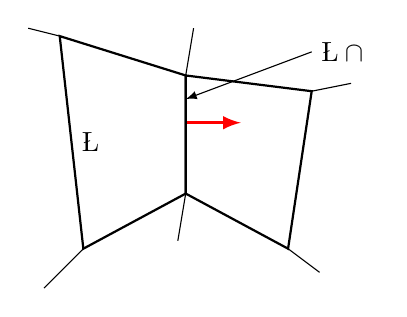
\begin{tikzpicture}[scale=1]
			\draw [arrows={-latex},very thick,red] (2,2.6)
				-- node[red, midway, below] {$\n$} (2.7,2.6); % normal
			\draw [thick] (0.7,1) -- node[midway, right] {$\L$} (0.4,3.7)
				-- (2,3.2) -- (2,1.7) -- cycle; % polygon L
			\draw [thick] (2,1.7) -- (2,3.2) -- (3.6,3)
				-- node[midway, left] {$\R$} (3.3,1) -- cycle; % polygon R
			\draw [arrows={-latex}] (3.6,3.5) node[right] {$\Bord{\L} \cap \Bord{\R}$}
				-- (2,2.9); % flèche interface
			\draw (0.7,1) -- (0.2,0.5); % arêtes sortantes
			\draw (0.4,3.7) -- (0,3.8);
			\draw (2,3.2) -- (2.1,3.8);
			\draw (3.6,3) -- (4.1,3.1);
			\draw (3.3,1) -- (3.7,0.7);
			\draw (2,1.7) -- (1.9,1.1);
		\end{tikzpicture}
	\end{center}
\end{figure}

Nous rappelons que les indices $\L$ et $\R$ font références aux ouverts situés de
chaque côté de $\UItf$ (figure \ref{img:cell_LR}). La surface $\UItf$ est orientée de telle sorte que
le vecteur normal unitaire à $\UItf$, noté $\n$, soit orienté de $\L$ vers $\R$.
Les champs $\W_\L$, respectivement $\W_\R$, sont la restriction à $\UItf$ des
champs provenant du côté $\L$, respectivement $\R$.
\\


\subsection{Formulation GD}
\label{ssect:formulation_gd}

Maintenant que nous avons établi une formulation faible du problème, nous pouvons
en déduire une formulation GD. Nous allons étendre la formulation
faible à des fonctions tests pouvant également présenter une discontinuité
sur les interfaces entre ouverts et ayant la même régularité que la solution.
Pour cela, nous introduisons un flux numérique, dépendant des états $\W_\L$ et
$\W_\R$ afin de donner un sens à l’intégrale sur $\UItf \setminus
\Bord{\PbEsp}$.
\\

Rappelons que dans le cas des équations de Maxwell,
la matrice $\Aini$ est symétrique et vaut :
\begin{align}
	\Aini = 
	\begin{pmatrix}
		0 & -\n \times \\
		\n \times & 0
	\end{pmatrix} ,
	\; \mathrm{avec} \;
	\n \times =
	\begin{pmatrix}
		0 & -\nC{3} & \nC{2} \\
		\nC{3} & 0 & -\nC{1} \\
		-\nC{2} & \nC{1} & 0
	\end{pmatrix} .
\end{align}
Les valeurs propres de cette matrice sont $\pm \Norm{\n}^2$ et $0$.
Dans le cas où le vecteur $\n$ est unitaire, les matrices $\Pos{\Aini}$ et
$\Neg{\Aini}$ sont elles aussi symétriques et valent :
\begin{subequations}
	\begin{align}
		\Pos{\Aini} &= \frac{1}{2}
		\begin{pmatrix}
			-(\n \times)^2 & -\n \times \\
			\n \times & -(\n \times)^2
		\end{pmatrix} ,
		\\
		\Neg{\Aini} &= \frac{1}{2}
		\begin{pmatrix}
			(\n \times)^2 & -\n \times \\
			\n \times & (\n \times)^2
		\end{pmatrix} .
	\end{align}
\end{subequations}
La matrice $(\n \times)^2$ correspond à l'application, sur un vecteur $\U$,
de l'opération $\n \times (\n \times \U)$. Nous avons :
\begin{align}
	(\n \times)^2 = \begin{pmatrix}
	- \nC{2}^2 - \nC{3}^2 & \nC{1} \nC{2} & \nC{3} \nC{1} \\
	\nC{1} \nC{2} & - \nC{3}^2 - \nC{1}^2 & \nC{2} \nC{3} \\
	\nC{3} \nC{1} & \nC{2} \nC{3} & - \nC{1}^2 - \nC{2}^2
	\end{pmatrix} .
\end{align}

Nous introduisons alors ces matrices dans la formulation faible
\eqref{eq:formulation_faible} et obtenons ainsi la formulation GD.
Pour toute fonction test $\psi$ éventuellement discontinue sur
$\UItf$ :
\begin{equation}
	\begin{aligned}
		\int_{\PbEsp} \Ptl{t} \W \psi d\x
		&+ \int_{\UElt} \Aidi \W \psi d\x \\
		&+ \int_{\UItf \setminus \Bord{\PbEsp}}
			\Neg{\Aini} (\W_\R - \W_\L) \psi_\L +
			\Pos{\Aini} (\W_\R - \W_\L) \psi_\R ds \\
		&+ \int_{\Bord{\PbEsp}} \MatB \W_\L \psi_\L ds = 0
		\label{eq:formulation_gd} .
	\end{aligned}
\end{equation}


Il est important de remarquer ici que cette formulation faible n’a plus de
sens dans l’espace des distributions $\mathcal{D}(\PbEsp)$ puisque
les fonctions tests sont
maintenant discontinues. Cette formulation a du sens par exemple lorsque $\W$
est de classe $\mathcal{C}^1$ sur toute cellule $\Adh{\L}$ du maillage $\Mesh$. Nous
pouvons donc introduire l’espace de fonctions suivant :
\begin{align}
	\mathcal{H} = \lbrace
		f \in \mathrm{L}^2(\PbEsp) :
		\forall \L \in \Mesh,
		f_{\vert \L} \in \mathcal{C}^1(\Adh{\L})
	\rbrace .
\end{align}

Nous cherchons alors la solution $\W$ dans $\mathcal{C}^1(\PbTps,\mathcal{H}^\NC)$.
Lorsque les fonctions tests s’annulent en dehors de $\Adh{\L}$, la formulation GD
\eqref{eq:formulation_gd} sur $\L$ devient :
\begin{equation}
	\begin{aligned}
		\int_{\L} \Ptl{t} \W \psi d\x 
		&+ \int_{\L} \Aidi \W \psi d\x \\
		&+ \int_{\Bord{\L} \setminus \Bord{\PbEsp}}
			\Neg{\Aini} (\W_\R - \W_\L) \psi_\L ds \\
		&+ \int_{\Bord{\L} \cap \Bord{\PbEsp}} \MatB \W_\L \psi_\L ds = 0
		\label{eq:formulation_gd_locale} .
	\end{aligned}
\end{equation}
En appliquant ensuite la formule de Green sur le second terme :
\begin{align}
	\int_{\L} \nabla \phi \psi =
	- \int_{\L} \nabla \psi \phi
	+ \int_{\Bord{\L}} \n \phi \psi
	\label{eq:formule_de_green} ,
\end{align}
l’équation précédente devient :
\begin{equation}
	\begin{aligned}
		\int_{\L} \Ptl{t} \W \psi d\x
		&- \int_{\L} \Aidi \psi \W d\x \\
		&+ \int_{\Bord{\L} \setminus \Bord{\PbEsp}}
			(\Pos{\Aini} \W_\L + \Neg{\Aini} \W_\R) \psi_\L ds \\
		&+ \int_{\Bord{\L} \cap \Bord{\PbEsp}}
			(\Aini + \MatB) \W_\L \psi_\L ds = 0
		\label{eq:formulation_gd_green} .
	\end{aligned}
\end{equation}


Nous introduisons alors le flux numérique :
\begin{align}
	\Flux{\W_\L}{\W_\R}{\n} = \Pos{\Aini} \W_\L + \Neg{\Aini} \W_\R
	\label{eq:flux_numerique}
\end{align}
et le flux de bord :
\begin{align}
	\FluxB{\W}{\n} = (\Aini + \MatB) \W
	\label{eq:flux_bord} .
\end{align}

Ce flux numérique est un flux décentré.
Nous avons choisi ce flux car il introduit une dissipation
numérique qui améliore la stabilité du schéma selon les travaux de
Castel \textit{et al.} \cite{castel:hal-00403787},
Cohen \textit{et al.} \cite{Coh-Fer-Per-2006-1} et
Hesthaven \textit{et al.} \cite{Hesthaven493}.

Pour obtenir une approximation convergente vers la bonne solution,
le flux doit vérifier les propriétés de consistance :
\begin{align}
	\Flux{\W}{\W}{\n} = \Aini \W
	\label{eq:flux_consistance}
\end{align}
et de conservation :
\begin{align}
	\Flux{\W_\L}{\W_\R}{-\n} = - \Flux{\W_\R}{\W_\L}{\n}
	\label{eq:flux_conservation} .
\end{align}

Il est possible de choisir d’autres flux numériques.
Dans le cas des équations de Maxwell, nous pouvons donner
une famille de flux numériques plus généraux, en fonction d’un paramètre
$\alpha \ge 0$, qui garantissent la stabilité
du schéma numérique :
\begin{align}
	\F_\alpha (\W_\L, \W_\R, \n) =
	\begin{pmatrix}
		- \frac{1}{2} \n \times (\H_\L + \H_\R)
		+ \alpha (\n \times)^2 (\E_\R - \E_\L) \\
		\frac{1}{2} \n \times (\E_\L + \E_\R)
		+ \alpha (\n \times)^2 (\H_\R - \H_\L)
	\end{pmatrix} .
\end{align}
Le paramètre $\alpha$ définit le décentrage du flux numérique et la
dissipation de l’énergie induite.
Lorsque $\alpha = \frac{1}{2}$, le flux est décentré.
Lorsque $\alpha = 0$, le flux est centré.

%  PH: faire une proposition qui montre que ces flux vérifient les deux propriétés ci-dessus: conservation et consistance
%  BW:
\begin{proposition}
	La famille de flux $\F_\alpha$ vérifie les
	propriétés de consistance \eqref{eq:flux_consistance}
	et de conservation \eqref{eq:flux_conservation}.
\end{proposition}
\begin{proof}
	Consistance :
	\begin{align}
		\F_\alpha (\W, \W, \n) =
		\begin{pmatrix}
			- \n \times \H \\
			\n \times \E
		\end{pmatrix} =
		\begin{pmatrix}
			0 & - \n \times \\
			\n \times & 0
		\end{pmatrix}
		\begin{pmatrix}
			\E \\
			\H
		\end{pmatrix} =
		\Aini \W .
	\end{align}
	Conservation :
	\begin{equation}
		\begin{aligned}
			- \F_\alpha (&\W_\L, \W_\R, -\n) \\ &=
			\begin{pmatrix}
				\frac{1}{2} (-\n) \times (\H_\L + \H_\R)
				- \alpha (-\n \times)^2 (\E_\R - \E_\L) \\
				- \frac{1}{2} (-\n) \times (\E_\L + \E_\R)
				- \alpha (-\n \times)^2 (\H_\R - \H_\L)
			\end{pmatrix} \\ &=
			\begin{pmatrix}
				- \frac{1}{2} \n \times (\H_\R + \H_\L)
				+ \alpha (\n \times)^2 (\E_\L - \E_\R) \\
				\frac{1}{2} \n \times (\E_\R + \E_\L)
				+ \alpha (\n \times)^2 (\H_\L - \H_\R)
			\end{pmatrix} \\
			&= \F_\alpha (\W_\R, \W_\L, \n) .
		\end{aligned}
	\end{equation}
\end{proof}

Nous obtenons finalement la formulation GD de notre problème : trouver
une solution $\W \in \mathcal{C}^1(\PbTps,\mathcal{H}^\NC)$ telle que :
\begin{equation}
	\begin{aligned}
		\forall \L \in \Mesh, \forall \psi \in \mathcal{C}^1(\Adh{\L}), \\
		\int_{\L} \Ptl{t} \W \psi d\x
		&- \int_{\L} \Flux{\W}{\W}{\nabla \psi} d\x \\
		&+ \int_{\Bord{\L} \setminus \Bord{\PbEsp}}
			\Flux{\W_\L}{\W_\R}{\n} \psi_\L ds \\
		&+ \int_{\Bord{\L} \cap \Bord{\PbEsp}}
			\FluxB{\W_\L}{\n} \psi_\L ds = 0
		\label{eq:formulation_gd_finale} .
	\end{aligned}
\end{equation}
En ajoutant à cette formulation un état initial $\W(0) = \Winit$,
le problème d’évolution ainsi posé admet en principe une unique solution.
\\


\subsection{Stabilité de la méthode}
\label{ssect:stabilite_gd}

Nous nous intéressons à présent à la stabilité de cette méthode. Plaçons-nous dans
le cas où aucune source d’énergie n’est placée dans le domaine. La méthode sera stable
si l’énergie du système décroit au cours du temps. Afin d’alléger les écritures,
supposons, sans perte de généralité, que la matrice $\At$ est égale à l’identité.
Dans la définition \ref{def:energie}, nous avons défini une énergie associée
à la solution $\W$.
En différenciant son expression par rapport au temps nous obtenons :
\begin{align}
	\Ptl{t} \Energy = \frac{1}{2} \int_{\PbEsp} \Ptl{t} \W \cdot \W d\x .
\end{align}

En prenant $\psi = \W$ dans la formulation GD \eqref{eq:formulation_gd} nous
pouvons exprimer la dérivée temporelle de l'énergie :
\begin{equation}
	\begin{aligned}
		\int_{\PbEsp} \Ptl{t} \W \cdot \W d\x =
		&- \int_{\UElt} (\Aidi \W) \cdot \W d\x \\
		&- \int_{\UItf \setminus \Bord{\PbEsp}}
			(\Neg{\Aini} (\W_\R - \W_\L)) \cdot \W_\L ds \\
		&- \int_{\UItf \setminus \Bord{\PbEsp}}
			(\Pos{\Aini} (\W_\R - \W_\L)) \cdot \W_\R ds \\
		&- \int_{\Bord{\PbEsp}} (\MatB \W_\L) \cdot \W_\L ds .
	\end{aligned}
\end{equation}

Le premier terme du membre de doite peut être décomposé comme suit :
\begin{equation}
	\begin{aligned}
		\int_{\UElt} &(\Aidi \W) \cdot \W d\x
		= \frac{1}{2} \int_{\UElt} \Ptl{i} ((\Ai \W) \cdot \W) d\x \\
		&= \frac{1}{2} \int_{\UItf} (\Aini \W_\L) \cdot \W_\L ds
		- \frac{1}{2} \int_{\UItf \setminus \Bord{\PbEsp}}
			(\Aini \W_\R) \cdot \W_\R ds\\
		&= \frac{1}{2} \int_{\Bord{\PbEsp}} (\Aini \W_\L) \cdot \W_\L ds
		+ \frac{1}{2} \int_{\UItf \setminus \Bord{\PbEsp}}
			(\Aini \W_\L) \cdot \W_\L ds \\
		&\quad - \frac{1}{2} \int_{\UItf \setminus \Bord{\PbEsp}}
			(\Aini \W_\R) \cdot \W_\R ds \\
		&= \frac{1}{2} \int_{\Bord{\PbEsp}} (\Aini \W_\L) \cdot \W_\L ds \\
		&\quad - \frac{1}{2} \int_{\UItf \setminus \Bord{\PbEsp}}
			(\Aini (\W_\R - \W_\L)) \cdot \W_\L ds \\
		&\quad - \frac{1}{2} \int_{\UItf \setminus \Bord{\PbEsp}}
			(\Aini (\W_\R - \W_\L)) \cdot \W_\R ds .
	\end{aligned}
\end{equation}
De plus,
\begin{equation}
	\begin{aligned}
		\frac{1}{2} \int_{\UItf \setminus \Bord{\PbEsp}}
			(\Aini (\W_\R &- \W_\L)) \cdot \W_\L ds
		- \int_{\UItf \setminus \Bord{\PbEsp}}
			(\Neg{\Aini} (\W_\R - \W_\L)) \cdot \W_\L ds \\
		&= \frac{1}{2} \int_{\UItf \setminus \Bord{\PbEsp}}
			\left( \Abs{\Aini} (\W_\R - \W_\L) \right) \cdot \W_\L ds
	\end{aligned}
\end{equation}
et
\begin{equation}
	\begin{aligned}
		\frac{1}{2} \int_{\UItf \setminus \Bord{\PbEsp}}
			(\Aini (\W_\R &- \W_\L)) \cdot \W_\R ds
		- \int_{\UItf \setminus \Bord{\PbEsp}}
			(\Pos{\Aini} (\W_\R - \W_\L)) \cdot \W_\R ds \\
		&= - \frac{1}{2} \int_{\UItf \setminus \Bord{\PbEsp}}
			\left( \Abs{\Aini} (\W_\R - \W_\L) \right) \cdot \W_\R ds
	\end{aligned}
\end{equation}
où $\Abs{\Aini} = \Pos{\Aini} - \Neg{\Aini}$ est une matrice dont les
valeurs propres sont des réels positifs.

Ainsi, nous obtenons une expression de l’évolution de l’énergie ne faisant
intervenir que des intégrales surfaciques :
\begin{equation}
	\begin{aligned}
		\int_{\PbEsp} \Ptl{t} \W \cdot \W d\x =
		&- \frac{1}{2} \int_{\UItf \setminus \Bord{\PbEsp}}
			\left( \Abs{\Aini} (\W_\R - \W_\L) \right)
			\cdot (\W_\R - \W_\L) ds \\
		&- \int_{\Bord{\PbEsp}}
			\left( \left( \frac{1}{2} \Aini + \MatB \right) \W_\L \right)
			\cdot \W_\L ds .
	\end{aligned}
\end{equation}


Cette expression de l’énergie nous permet alors d’énoncer un théorème donnant
une condition suffisante de stabilité portant sur les conditions aux limites.
\begin{theorem} \label{thm:decroissance_energie}
	L'énergie $\Energy$ du système décroit si la matrice
	$\frac{1}{2} \Aini + \MatB$ est positive.
\end{theorem}

\begin{proof}
	La dérivée en temps de l’énergie vérifie
	\begin{equation}
		\begin{aligned}
			2 \Ptl{t} \Energy =
			&- \frac{1}{2} \int_{\UItf \setminus \Bord{\PbEsp}}
				\left( \Abs{\Aini} (\W_\R - \W_\L) \right)
				\cdot (\W_\R - \W_\L) ds \\
			&- \int_{\Bord{\PbEsp}}
				\left( \left( \frac{1}{2} \Aini + \MatB \right) \W_\L \right)
				\cdot \W_\L ds .
		\end{aligned}
	\end{equation}
	Puisque la matrice $\Abs{\Aini}$ est une matrice positive, si la matrice
	$\frac{1}{2} \Aini + \MatB$ est aussi positive, les intégrales de cette équation sont
	positives pour tout $\W \in \mathcal{H}^\NC$.
	Dans ce cas la dérivée en temps de $\Energy$ est négative et donc $\Energy$ décroit.
\end{proof}

\begin{remark}
	Cette condition de stabilité porte sur l’expression des conditions aux limites
	utilisées dans la formulation GD. En particulier, ce théorème nous permettra
	de déduire d’une condition « physique », la (ou les) matrice(s) $\MatB$ la représentant
	et garantissant la stabilité du schéma en découlant.
\end{remark}

\begin{remark}
	Si la condition de stabilité est vérifiée, alors le théorème assurant l’unicité
	de la solution (théorème \ref{thm:unicite}) est vérifié. En effet,
	\begin{align}
		\forall \W \in \ker \MatB, \;
		0 \le \left( \left( \frac{1}{2} \Aini + \MatB \right) \W \right) \cdot \W
		= \frac{1}{2} (\Aini \W) \cdot \W .
	\end{align}
	\\
\end{remark}


\subsection{Formulation semi-discrète}
\label{ssect:formulation_semi-discrete}


Supposons maintenant que nous avons construit un maillage $\Mesh$ de $\PbEsp$
dont les bords des mailles correspondent exactement aux discontinuités stationnaires
de la solution exacte. Nous approximons alors la solution $\W$ du système de
Friedrichs \eqref{eq:friedrichs} par une solution discrète $\Wd$ dont les composantes
à chaque instant $t$ sont polynomiales de degré $\Deg$ dans chaque maille.
Ces fonctions polynomiales forment un espace vectoriel de dimension $p$ engendré par la base
$(\PsiPhy{\L}{i})_{i \in \Range{0}{p-1}}$.
Par exemple, cette base pourrait être constituée de produits tensoriels de polynômes
de degré au plus $\Deg$, nous décrirons plus loin un tel espace d’approximation. Notons
alors cet espace d’approximation :
\begin{align} \label{eq:ev_solution_discrete}
	\mathcal{H}_h = \mathrm{vect} \lbrace
		\PsiPhy{\L}{i} : \L \in \Mesh, \; i \in \Range{0}{p-1}
	\rbrace .
\end{align}
Le paramètre $h$ représente un paramètre de finesse du maillage, par exemple
le diamètre maximal des mailles. Les fonctions $\PsiPhy{\L}{i}$ sont nulles
en dehors de la maille $\L$. Elles constituent une base de dimension finie
de fonctions définies sur $\L$.

%  PH: vecteur en gras ? si ou tous les mettre, sinon n'en mettre aucun !
%  BW: choix d'une notation en gras jusqu'à après démonstration de convergence
Sur la maille $\L$, nous avons :
\begin{align}
	\forall \x \in \L, \;
	\W(\x,t) \approx \Wd(\x,t) = \sum_{i=0}^{p-1} \Wd_{\L,i}(t) \PsiPhy{\L}{i}(\x) .
\end{align}
Le problème semi-discret s’écrit alors comme suit.

Trouver une solution $\Wd \in \mathcal{C}^1(\PbTps,\mathcal{H}_h^\NC)$ telle que :
\begin{equation}
	\begin{aligned}
		\forall \L \in \Mesh, \;
		\forall \psi &\in \mathcal{H}_h : \mathrm{supp}(\psi) \subset \Adh{\L}, \\
		\int_{\L} \Ptl{t} \Wd \psi d\x
		&- \int_{\L} \Flux{\Wd}{\Wd}{\nabla \psi} d\x \\
		&+ \int_{\Bord{\L} \setminus \Bord{\PbEsp}}
			\Flux{\Wd_\L}{\Wd_\R}{\n} \psi_\L ds \\
		&+ \int_{\Bord{\L} \cap \Bord{\PbEsp}}
			\FluxB{\Wd_\L}{\n} \psi_\L ds = 0
		\label{eq:formulation_semi-discrete} .
	\end{aligned}
\end{equation}


\begin{theorem} \label{thm:convergence_pb_discret}
	La solution du problème semi-discret \eqref{eq:formulation_semi-discrete}
	converge vers la solution du problème continu \eqref{eq:probleme_evolution}
	lorsque $h$ tend vers zéro.
\end{theorem}

Nous ne démontrerons pas ce théorème ici. Dans un souci de 
complétude, la démonstration est donnée en annexe \ref{annexe:demo_cv}.
\\

A présent que le théorème de convergence du problème semi-discret est énoncé,
nous pouvons identifier la solution discrète à la solution exacte
dans la suite en utilisant l'abus de notation $\Wd = \W$.
\\



\section*{Conclusion}

Dans ce premier chapitre, nous avons rappelé
les équations de Maxwell et montré qu’elles constituent un système
hyperbolique dit de Friedrichs.
En plus de ce système hyperbolique, le modèle de Maxwell donne
une condition initiale sur la divergence des champs.

Nous avons ensuite présenté la méthode GD, particulièrement bien adaptée
à la résolution de champs réguliers présentant
des discontinuités sur des interfaces stationnaires.
Cette méthode peut être appliquée à tout système de Friedrichs.
Elle fait intervenir un flux numérique que nous avons choisi décentré
afin d'améliorer la stabilité du schéma.
Nous avons également caractérisé les
conditions limites permettant d’assurer cette stabilité.

Enfin, nous avons déduit de cette formulation GD une formulation semi-discrète dont la solution converge vers celle du problème continu.
De plus, cette formulation prend naturellement en compte les discontinuités de la solution.
\\

Dans le chapitre suivant, nous appliquerons la condition de stabilité du théorème \ref{thm:decroissance_energie}
afin de valider différentes conditions aux limites présentes dans
la littérature et associées aux équations de Maxwell.
Nous donnerons aussi quelques modèles de simulation
fréquemment utilisés et dont nous aurons besoin dans nos cas d'application.


